\section{Polsby-Popper}\label{sec:pp}
The final compactness score we analyze is the \textit{Polsby-Popper
score}, which takes the form of an \textit{isoperimetric quotient},
meaning it measures how much area a region's perimeter encloses,
relative to all other regions with the same perimeter.

\begin{definition}\label{def:pp}
  The Polsby-Popper score of a region $\Omega$ is defined to be
  $$\mathrm{PP}(\Omega) = \frac{4\pi
  \cdot\mathrm{area}(\Omega)}{\mathrm{perim}(\Omega)^2}$$ 
in either the sphere or the plane, and
  $\mathrm{area}$ and $\mathrm{perim}$ are the area and perimeter of
    $\Omega$, respectively.
\end{definition}

The ancient Greeks were first to observe that if $\Omega$ is a region
in the plane, then $4\pi\cdot\mathrm{area}(\Omega)\leq
\mathrm{perim}(\Omega)^2$, with equality if and only if $\Omega$ is
a circle. This became known as the \textit{isoperimetric inequality} in
the plane.  This means that, in the plane, $0\le \mathrm{PP}(\Omega)\le 1$,
where the Polsby-Popper score is equal to $1$ only in the case of
a circle. We can observe that the Polsby-Popper score is scale-invariant in
the plane. 

An isoperimetric inequality for the sphere exists, and we
state it as the following lemma.  For a more detailed treatment of
isoperimetry in general, see \cite{osserman1979bonnesen}, and for
a proof of this inequality for the sphere, see \cite{rado}.

\begin{lemma}
  If $\Omega$ is a region on the sphere with area
  $A$ and perimeter $P$, then $P^2\geq 4\pi A - A^2$ with equality if
  and only if $\Omega$ is a spherical cap.
\end{lemma}
A consequence of this is that among all regions on the sphere with
a fixed area $A$, a spherical cap with area $A$ has the shortest
perimeter. However, the key difference between the Polsby-Popper score in the plane and on the sphere is that on the 
sphere, there is no scale invariance; two spherical caps of different sizes will have different scores.


\begin{lemma}\label{lem:ppscale}
  Let $S$ be the unit sphere, and let $\kappa(h)$ be a cap of height
  $h$.  Then $\mathrm{PP}(\kappa(h))$ is
  a monotonically increasing function of $h$.
\end{lemma}


\begin{proof}
  Let $r(h)$ be the radius of the circle bounding $\kappa(h)$. We
  compute: 
  \begin{align*}
    1 &= r(h)^2 + (1-h)^2 \text {, by right triangle trigonometry}\\ 
      &= r(h)^2 + 1 - 2h+h^2
  \end{align*}
  Rearranging, we get that $r(h)^2= 2h-h^2$, which we can plug in to
  the standard formula for perimeter:
  \begin{align*}
    \mathrm{perim}_S(\kappa(h)) = 2\pi r(h) = 2\pi \sqrt{2h-h^2}
  \end{align*}
  We can now use the Archimedian equal-area projection 
  defined by $(x,y,z) \to
  \left(\frac{x}{\sqrt{x^2+y^2}},\frac{y}{\sqrt{x^2+y^2}}, z\right)$ 
  to compute $\mathrm{area}_S(\kappa(h)) = 2\pi h$ and plug it in to 
  get:

  \begin{align*}
    \mathrm{PP}_S(\kappa(h)) = \frac{4\pi (2\pi h) }{4 \pi^2 (2h-h^2)}
    = \frac{2}{2-h}
  \end{align*}
  Which is a monotonically increasing function of $h$.
\end{proof}
\begin{corollary}\label{cor:capscale}
  On the sphere, Polsby-Popper scores of caps are monotonically
  increasing with area,
\end{corollary}
Using this, we can show the main theorem of this section, that no map
projection from a region on the sphere to the plane can preserve the ordering
of Polsby-Popper scores for all regions.  

\begin{theorem}\label{thm:dpp}
  If $\varphi:U\to V$ is a map projection from the sphere to the plane,
  then there exist two regions $A,B\subset U$ such that
  the Polsby-Popper score of $B$ is greater than that of $A$ in the
  sphere, but the Polsby-Popper score of $\varphi(A)$ is greater than
  that of $\varphi(B)$ in the plane.
\end{theorem}
\begin{figure}[h]
  \centering
  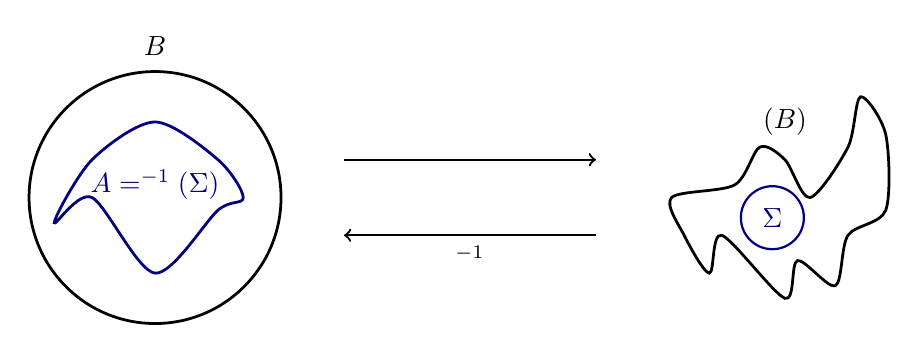
\begin{tikzpicture}[scale=1.6]
    \draw[thick,->] (-1,0.3)-- (1,0.3)%
    node[midway,above] {$\vphi$};
    \draw[thick,->] (1,-0.3) -- (-1,-0.3)%
    node[midway,below] {$\vphi^{-1}$}; 
    \draw[line width=1, black] (-2.5,0) circle (1);
    \draw node at (-2.5,1.2) {\color{black} $B$};
    \draw[line width=1, black] plot [smooth cycle, tension=0.5]%
    coordinates { (2.5,-0.8) (2.6,-0.5) (2.9,-0.7) (3,-0.3) (3.3,-0.1)% 
    (3.3,0.5) (3.1,0.8) (3,0.4) (2.7,0) (2.5,0.3) (2.3,0.4)%
    (2.1,0.1) (1.6,0) (1.7,-0.3) (1.9, -0.6) (2,-0.3)};
    \draw node at (2.5,0.6) {\color{black} $\vphi(B)$};

    \draw[thick, NavyBlue] (2.4,-0.16) circle (0.25);
    \draw node at (2.4,-0.16) {\color{NavyBlue} $\Sigma$};
    \draw[line width=1, NavyBlue] plot [smooth cycle, tension=0.5]%
    coordinates { (-2.5,-0.6) (-3, 0) (-3.3,-0.2) (-3,0.3) (-2.5,0.6)%
    (-2,0.3) (-1.8,0) (-2,-0.1)};
    \draw node at (-2.5,0.1) {\color{NavyBlue} $A=\vphi^{-1}(\Sigma)$};
  \end{tikzpicture}
  \caption{The construction of regions $A$, and $B$ in the
  proof of Theorem~\ref{thm:dpp}.} 
\label{fig:dpp}
\end{figure}

\begin{proof}
  Let $\varphi$ be a map projection, and let 
  $\kappa \subset U$ be some cap. We will take our regions 
  $A$ and $B$ to lie in $\kappa$. Set $B$ to be a cap 
  contained in $\kappa$. Let $\Sigma$ be a circle in 
  the plane such that $\Sigma
  \subsetneq \varphi(B)$ and let $A=\varphi^{-1}(\Sigma)$ (see
  Figure~\ref{fig:dpp}).

  We now use the isoperimetric inequality for the sphere 
  and Corollary~\ref{cor:capscale} to claim that 
  $A$ does not maximize the Polsby-Popper score in the sphere.

  To see this, take $\hat{A}$ to be a cap in the sphere with 
  area equal to that of $A$. Note that since the 
  area of $\hat {A}$ is less than the area of the cap $B$, it 
  follows that we can choose $\hat{A}\subset B$. 
  
  By the isoperimetric inequality of the sphere, 
  $\mathrm{PP}_S(\hat{A})\geq
  \mathrm{PP}_S(A)$. Since map projections preserve containment,
  $\Sigma\subsetneq \varphi(B)$ implies that $A\subsetneq B$, 
  meaning that $\mathrm{area}(\hat A) = \mathrm{area}(A)\lneq 
  \mathrm{area}(B)$. By Corollary~\ref{cor:capscale}, we know that
  $\mathrm{PP_S}(\hat{A})< \mathrm{PP_S}(B)$, and combining this with
  the earlier inequality, we get
  \begin{align*}
    \mathrm{PP_S}({A})\leq \mathrm{PP_S}(\hat{A})< \mathrm{PP_S}(B)
  \end{align*}

  Since $\Sigma = \varphi(A)$ maximizes the Polsby-Popper score in the
  plane, but $A$ does not do so in the sphere, we have shown that
  $\varphi$ does not preserve the maximal elements in the score
  ordering, and therefore it cannot preserve the ordering itself.
\end{proof}

The reason why every map projection fails to preserve the ordering of
Polsby-Popper scores is because the score itself is constructed from
the \textit{planar} notion of isoperimetry, and there is no reason to
expect this formula to move nicely back and forth between the sphere
and the plane.  This proof crucially exploits a scale invariance
present in the plane but not the sphere.  If we consider any circle in
the plane, its Polsby-Popper score is equal to one,
but that is not true of every cap in the sphere.  \mute{This naturally
raises the question of whether being more careful, and defining
a compactness score which uses the isoperimetric quotient of the
surface the region is actually in will evade this problem.  We show
later that it does resolve the issue of scale-noninvariance, but it is
still induces an ordering which is not preserved by any map
projection.  We discuss this further in \Cref{sec:generalz}.}
